
\subsubsection{11.11.14}

\begin{enumerate} 
	\item Time of beginning and ending of congregation:
	17:00 - 20:30
	\item Purposes of congregation:
	\begin{enumerate}
		\item Finish MCB.
		
		\item Add to programme of control of robot control of MCB.
		
		\item Write the programme of control of robot with two joysticks.
		
	\end{enumerate}
	
	\item Work, that has been done:
	\begin{enumerate}
		\item MCB was finished.
		
		\begin{figure}[H]
			\begin{minipage}[h]{0.47\linewidth}
				\center{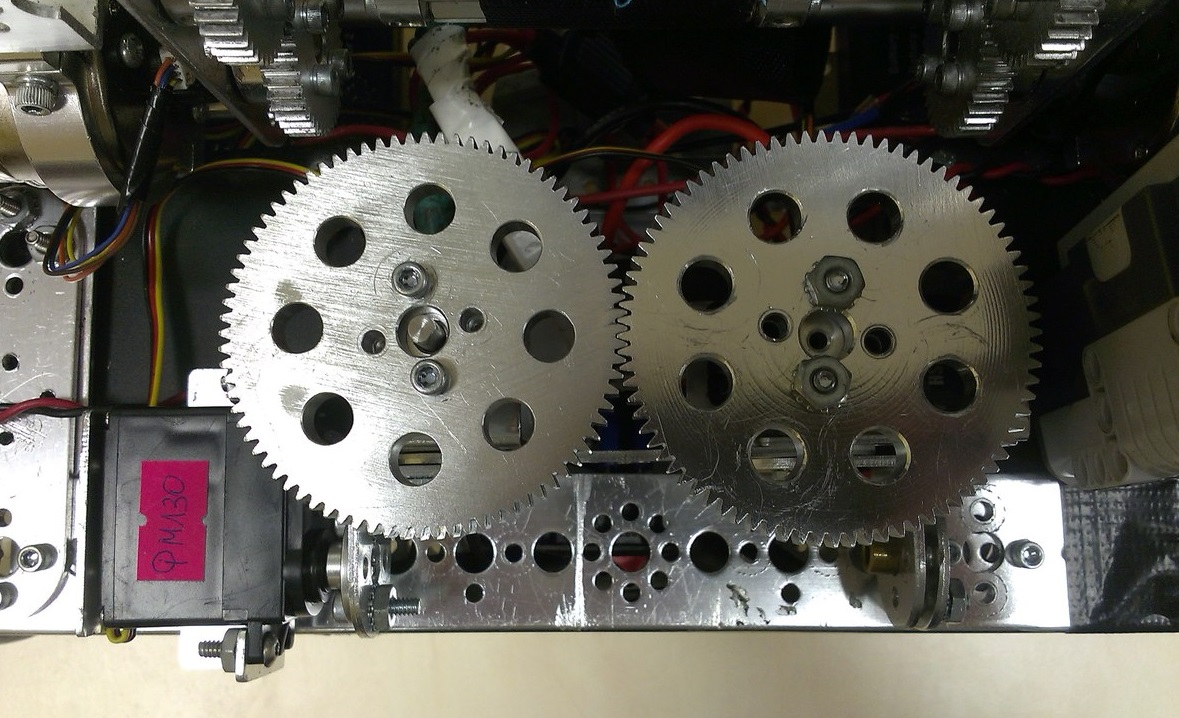
\includegraphics[scale=0.2]{days/11.11.14/images/01}}  
			\end{minipage}
			\begin{minipage}[h]{0.47\linewidth}
				\center{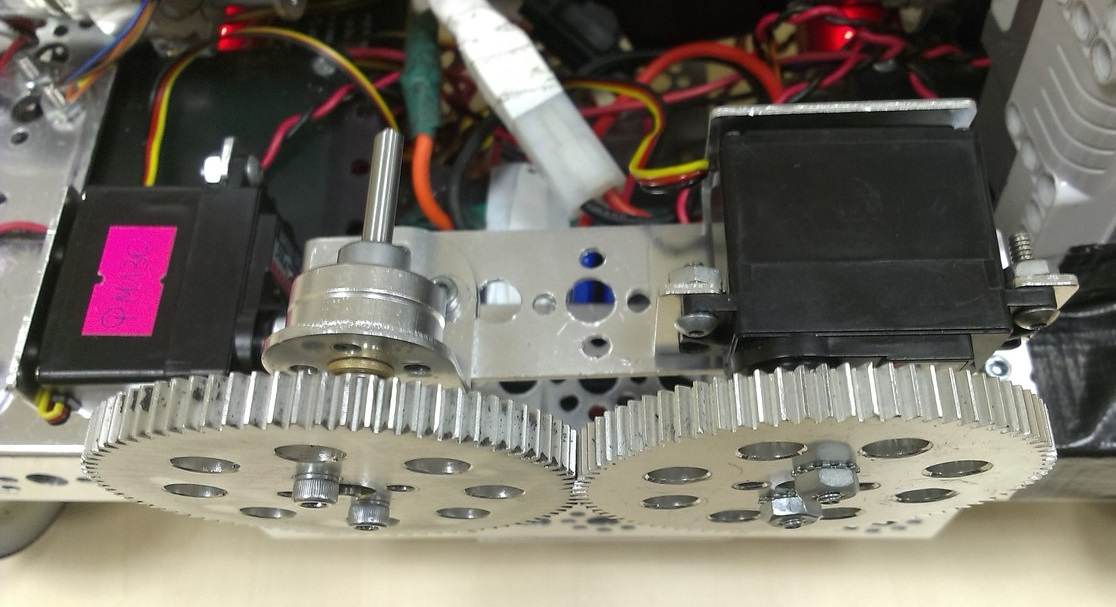
\includegraphics[scale=0.2]{days/11.11.14/images/02}}
			\end{minipage}
			\caption{Finished MCB}
		\end{figure}
		
		\item Programme of control MCB is not implemented.
		
		\item Today it was chosen the place for NXT. Now it was fixed by scotch but we planned to fix it more reliable.
		
		\begin{figure}[H]
			\begin{minipage}[h]{0.2\linewidth}
				\center  
			\end{minipage}
			\begin{minipage}[h]{0.6\linewidth}
				\center{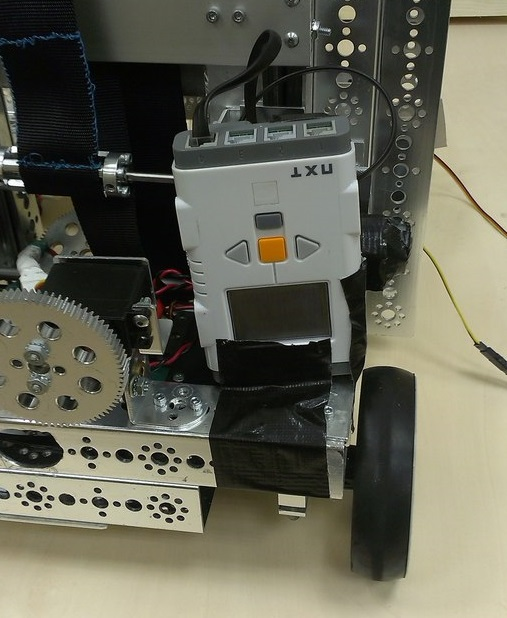
\includegraphics[scale=0.3]{days/11.11.14/images/03}}
				\caption{Place for mount of NXT}
			\end{minipage}
		\end{figure}
		
		\item We noticed to the fact that the wire of servo that tips the bucket touches the floor when lift is folded. It can to prevent of bucket's moving. It was decided to create special coil that working on the principle of roulette and uncoil wire when it is not in tension or fix the wire in several places at the guides of lift.
		
		\item Due to the fact that sometimes we need to test one of the nodes of robot or rotate motors which hard to turn by arms, for example for repair or replacement of elements, it was decided to create a special programme which allows to us control one of the nodes of robot by NXT's buttons, without control of a robot with joystick.
		
		\item The programme of control with two joysticks was created but wasn't tested. In the new programme the first operator responsible for everything, except moving, and the second responsible for moving.
		
		\item It was elaborated the mechanism of the churning stops from the central goal in autonomous period: at the robot must be installed servo of continuous rotation at which will fixed two chains of beams from set Lego-NXT, joined together, so every two beams connected by one pin. When it folded this construction doesn't take up much space but when servo starts rotation it will be straight, so for churning stops, it will enough to pass from him in the distance of action of mechanism. It more easy than write programme of finding of stop by IR sensor.
		
		\begin{figure}[H]
			\begin{minipage}[h]{0.2\linewidth}
				\center  
			\end{minipage}
			\begin{minipage}[h]{0.6\linewidth}
				\center{
\includegraphics[scale=0.2]{days/11.11.14/images/04}}
				\caption{Idea of mechanism of churing the stop}
			\end{minipage}
		\end{figure}
		
	\end{enumerate}
	
	\item Results:  
	\begin{enumerate}
		\item MCB almost finished.
		
		\item Programme of control MCB wasn't implemented.
		
		\item Programme of control robot with two joysticks was created.
		
		\item NXT was fixed at the robot.
		
		\item It was elaborated concept of mechanism of churing of the stops.
		
	\end{enumerate}
	
	\item Tasks for the next congregations:
	\begin{enumerate}
		\item Test programme of control robot with two joysticks.
		
		\item Include to the programme of control robot  the control MCB.
		
		\item Fix the wire of servo, that turn bucket (hereinafter it will call STB) so that it doesn't prevent to moving of lift and bucket.
		
		\item Make the programme of control nodes of robot by buttons of NXT.
		
		\item Create and test the mechanism of churing of the stop.
		
	\end{enumerate}     
\end{enumerate}
\fillpage

